\subsection{Versuch 1}
\begin{frame}
Auswirkung der Position im Raum auf die Berechnung und horizontaler Arbeitsbereich
\begin{itemize}
	\item<1-> Probanden befinden sich auf einem $1\times 1m$ Raster.
	\item<1-> $2688\times 1520$ Farbkamera mit $170^\circ$ Weitwinkel-Linse und großer Schärfentiefe.
	\item<1-> Blick-Ziel sind weit verteilt an der Wand
\end{itemize}
\begin{figure}
	\centering
	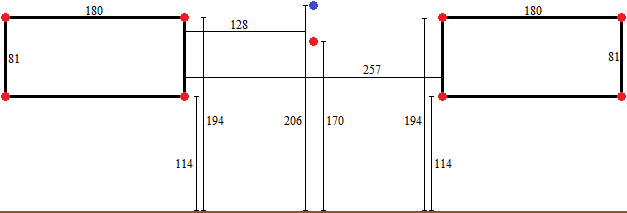
\includegraphics[width=0.7\linewidth]{images/Target}
\end{figure}
\end{frame}
\begin{frame}
\begin{center}
	\begin{tabular}{|c|c|c|c|c|c|}
	\hline 
	$+6m$ & &&&&\\
	\hline 
	$+5m$ &
	
\includegraphics[width=0.5cm]{img_Bereich/V1_img_Winkel_X_-2000_5000.png} &
	
\includegraphics[width=0.5cm]{img_Bereich/V1_img_Winkel_X_-1000_5000.png} &
	
\includegraphics[width=0.5cm]{img_Bereich/V1_img_Winkel_X_0_5000.png} &
	
\includegraphics[width=0.5cm]{img_Bereich/V1_img_Winkel_X_1000_5000.png} &
	
\includegraphics[width=0.5cm]{img_Bereich/V1_img_Winkel_X_2000_5000.png} \\ 
	\hline 
	$+4m$ &
	
\includegraphics[width=0.5cm]{img_Bereich/V1_img_Winkel_X_-2000_4000.png} &
	
\includegraphics[width=0.5cm]{img_Bereich/V1_img_Winkel_X_-1000_4000.png} &
	
\includegraphics[width=0.5cm]{img_Bereich/V1_img_Winkel_X_0_4000.png} &
	
\includegraphics[width=0.5cm]{img_Bereich/V1_img_Winkel_X_1000_4000.png} &
	
\includegraphics[width=0.5cm]{img_Bereich/V1_img_Winkel_X_2000_4000.png} \\ 
	\hline 
	$+3m$ &
	
\includegraphics[width=0.5cm]{img_Bereich/V1_img_Winkel_X_-2000_3000.png} &
	
\includegraphics[width=0.5cm]{img_Bereich/V1_img_Winkel_X_-1000_3000.png} &
	
\includegraphics[width=0.5cm]{img_Bereich/V1_img_Winkel_X_0_3000.png} &
	
\includegraphics[width=0.5cm]{img_Bereich/V1_img_Winkel_X_1000_3000.png} &
	
\includegraphics[width=0.5cm]{img_Bereich/V1_img_Winkel_X_2000_3000.png} \\ 
	\hline 
	$+2m$ &&
	
\includegraphics[width=0.5cm]{img_Bereich/V1_img_Winkel_X_-1000_2000.png} &
	
\includegraphics[width=0.5cm]{img_Bereich/V1_img_Winkel_X_0_2000.png} &
	
\includegraphics[width=0.5cm]{img_Bereich/V1_img_Winkel_X_1000_2000.png} & \\ 
	\hline 
	$+1m$ & &
	
\includegraphics[width=0.5cm]{img_Bereich/V1_img_Winkel_X_-1000_1000.png} &
	
\includegraphics[width=0.5cm]{img_Bereich/V1_img_Winkel_X_0_1000.png} &
	
\includegraphics[width=0.5cm]{img_Bereich/V1_img_Winkel_X_1000_1000.png} & \\ 
	\hline 
	& $-2m$ & $-1m$ &0& $+1m$ & $+2m$ \\ 
	\hline 
\end{tabular}
	\begin{tabular}{|c|c|c|c|c|c|c|c|}
	\hline
	$+6$ &
	
\includegraphics[width=0.045\linewidth]{img_Bereich/V1_vid_Winkel_X_-3000_5000.png}&
	
\includegraphics[width=0.045\linewidth]{img_Bereich/V1_vid_Winkel_X_-2000_5000.png}&
	
\includegraphics[width=0.045\linewidth]{img_Bereich/V1_vid_Winkel_X_-1000_5000.png}&
	
\includegraphics[width=0.045\linewidth]{img_Bereich/V1_vid_Winkel_X_0_5000.png}&
	
\includegraphics[width=0.045\linewidth]{img_Bereich/V1_vid_Winkel_X_1000_5000.png}&
	
\includegraphics[width=0.045\linewidth]{img_Bereich/V1_vid_Winkel_X_2000_5000.png}&\\ 
	\hline 
	$+5$ &
	
\includegraphics[width=0.045\linewidth]{img_Bereich/V1_vid_Winkel_X_-3000_5000.png}&
	
\includegraphics[width=0.045\linewidth]{img_Bereich/V1_vid_Winkel_X_-2000_5000.png}&
	
\includegraphics[width=0.045\linewidth]{img_Bereich/V1_vid_Winkel_X_-1000_5000.png}&
	
\includegraphics[width=0.045\linewidth]{img_Bereich/V1_vid_Winkel_X_0_5000.png}&
	
\includegraphics[width=0.045\linewidth]{img_Bereich/V1_vid_Winkel_X_1000_5000.png}&
	
\includegraphics[width=0.045\linewidth]{img_Bereich/V1_vid_Winkel_X_2000_5000.png}&\\ 
	\hline 
	$+4$ &
	
\includegraphics[width=0.045\linewidth]{img_Bereich/V1_vid_Winkel_X_-3000_4000.png}&
	
\includegraphics[width=0.045\linewidth]{img_Bereich/V1_vid_Winkel_X_-2000_4000.png}&
	
\includegraphics[width=0.045\linewidth]{img_Bereich/V1_vid_Winkel_X_-1000_4000.png}&
	
\includegraphics[width=0.045\linewidth]{img_Bereich/V1_vid_Winkel_X_0_4000.png}&
	
\includegraphics[width=0.045\linewidth]{img_Bereich/V1_vid_Winkel_X_1000_4000.png}&
	
\includegraphics[width=0.045\linewidth]{img_Bereich/V1_vid_Winkel_X_2000_4000.png}&
	
\includegraphics[width=0.045\linewidth]{img_Bereich/V1_vid_Winkel_X_3000_4000.png}\\ 
	\hline 
	$+3$ &
	
\includegraphics[width=0.045\linewidth]{img_Bereich/V1_vid_Winkel_X_-3000_3000.png}&
	
\includegraphics[width=0.045\linewidth]{img_Bereich/V1_vid_Winkel_X_-2000_3000.png}&
	
\includegraphics[width=0.045\linewidth]{img_Bereich/V1_vid_Winkel_X_-1000_3000.png}&
	
\includegraphics[width=0.045\linewidth]{img_Bereich/V1_vid_Winkel_X_0_3000.png}&
	
\includegraphics[width=0.045\linewidth]{img_Bereich/V1_vid_Winkel_X_1000_3000.png}&
	
\includegraphics[width=0.045\linewidth]{img_Bereich/V1_vid_Winkel_X_2000_3000.png}&
	
\includegraphics[width=0.045\linewidth]{img_Bereich/V1_vid_Winkel_X_3000_3000.png}\\ 
	\hline 
	$+2$ & &
	
\includegraphics[width=0.045\linewidth]{img_Bereich/V1_vid_Winkel_X_-2000_2000.png}&
	
\includegraphics[width=0.045\linewidth]{img_Bereich/V1_vid_Winkel_X_-1000_2000.png}&
	\includegraphics[width=0.045\linewidth]{img_Bereich/V1_vid_Winkel_X_0_2000.png}&
	\includegraphics[width=0.045\linewidth]{img_Bereich/V1_vid_Winkel_X_1000_2000.png}&
	\includegraphics[width=0.045\linewidth]{img_Bereich/V1_vid_Winkel_X_2000_2000.png}& \\ 
	\hline 
	$+1$ & & &
	\includegraphics[width=0.045\linewidth]{img_Bereich/V1_vid_Winkel_X_-1000_1000.png}&
	\includegraphics[width=0.045\linewidth]{img_Bereich/V1_vid_Winkel_X_0_1000.png}&
	\includegraphics[width=0.045\linewidth]{img_Bereich/V1_vid_Winkel_X_1000_1000.png}& &\\ 
	\hline 
	& $-3$& $-2$ & $-1$ &0& $+1$ & $+2$ & $+3$ \\ 
	\hline 
\end{tabular}
\end{center}
\end{frame}
\begin{frame}
\begin{center}
\begin{tabular}{|c|c|c|c|c|c|c|c|}
	\hline
	$+11m$ & & & &
	\includegraphics[width=1cm]{img_Bereich/V1_vid_res_Winkel_X_0_11000.png}& & &\\ 
	\hline 
	$+10m$ & & &
	\includegraphics[width=1cm]{img_Bereich/V1_vid_res_Winkel_X_-1000_10000.png}&
	\includegraphics[width=1cm]{img_Bereich/V1_vid_res_Winkel_X_0_10000.png}&
	\includegraphics[width=1cm]{img_Bereich/V1_vid_res_Winkel_X_1000_10000.png}&
	\includegraphics[width=1cm]{img_Bereich/V1_vid_res_Winkel_X_2000_10000.png}&\\ 
	\hline 
	$+9m$ & & &
	\includegraphics[width=1cm]{img_Bereich/V1_vid_res_Winkel_X_-1000_9000.png}&
	\includegraphics[width=1cm]{img_Bereich/V1_vid_res_Winkel_X_0_9000.png}&
	\includegraphics[width=1cm]{img_Bereich/V1_vid_res_Winkel_X_1000_9000.png}&
	\includegraphics[width=1cm]{img_Bereich/V1_vid_res_Winkel_X_2000_9000.png}&\\ 
	\hline 
	$+8m$ & & &
	\includegraphics[width=1cm]{img_Bereich/V1_vid_res_Winkel_X_-1000_8000.png}&
	\includegraphics[width=1cm]{img_Bereich/V1_vid_res_Winkel_X_0_8000.png}&
	\includegraphics[width=1cm]{img_Bereich/V1_vid_res_Winkel_X_1000_8000.png}& & \\ 
	\hline 
	$+7m$ & & &
	\includegraphics[width=1cm]{img_Bereich/V1_vid_res_Winkel_X_-1000_7000.png}&
	\includegraphics[width=1cm]{img_Bereich/V1_vid_res_Winkel_X_0_7000.png}&
	\includegraphics[width=1cm]{img_Bereich/V1_vid_res_Winkel_X_1000_7000.png}& & \\ 
	\hline 
	$+6m$ & & &
	\includegraphics[width=1cm]{img_Bereich/V1_vid_res_Winkel_X_-1000_6000.png}&
	\includegraphics[width=1cm]{img_Bereich/V1_vid_res_Winkel_X_0_6000.png}&
	\includegraphics[width=1cm]{img_Bereich/V1_vid_res_Winkel_X_1000_6000.png}&
	\includegraphics[width=1cm]{img_Bereich/V1_vid_res_Winkel_X_2000_6000.png}&
	\includegraphics[width=1cm]{img_Bereich/V1_vid_res_Winkel_X_3000_6000.png}\\ 
	\hline 
	$+5m$ &
	\includegraphics[width=1cm]{img_Bereich/V1_vid_res_Winkel_X_-3000_5000.png}& &
	\includegraphics[width=1cm]{img_Bereich/V1_vid_res_Winkel_X_-1000_5000.png}&
	\includegraphics[width=1cm]{img_Bereich/V1_vid_res_Winkel_X_0_5000.png}&
	\includegraphics[width=1cm]{img_Bereich/V1_vid_res_Winkel_X_1000_5000.png}&
	\includegraphics[width=1cm]{img_Bereich/V1_vid_res_Winkel_X_2000_5000.png}&
	\includegraphics[width=1cm]{img_Bereich/V1_vid_res_Winkel_X_3000_5000.png}\\ 
	\hline 
	$+4m$ &
	\includegraphics[width=1cm]{img_Bereich/V1_vid_res_Winkel_X_-3000_4000.png}& &
	\includegraphics[width=1cm]{img_Bereich/V1_vid_res_Winkel_X_-1000_4000.png}&
	\includegraphics[width=1cm]{img_Bereich/V1_vid_res_Winkel_X_0_4000.png}&
	\includegraphics[width=1cm]{img_Bereich/V1_vid_res_Winkel_X_1000_4000.png}&
	\includegraphics[width=1cm]{img_Bereich/V1_vid_res_Winkel_X_2000_4000.png}&
	\includegraphics[width=1cm]{img_Bereich/V1_vid_res_Winkel_X_3000_4000.png}\\ 
	\hline 
	$+3m$ &
	\includegraphics[width=1cm]{img_Bereich/V1_vid_res_Winkel_X_-3000_3000.png}& &
	\includegraphics[width=1cm]{img_Bereich/V1_vid_res_Winkel_X_-1000_3000.png}&
	\includegraphics[width=1cm]{img_Bereich/V1_vid_res_Winkel_X_0_3000.png}&
	\includegraphics[width=1cm]{img_Bereich/V1_vid_res_Winkel_X_1000_3000.png}&
	\includegraphics[width=1cm]{img_Bereich/V1_vid_res_Winkel_X_2000_3000.png}&
	\includegraphics[width=1cm]{img_Bereich/V1_vid_res_Winkel_X_3000_3000.png}\\ 
	\hline 
	$+2m$ & & &
	\includegraphics[width=1cm]{img_Bereich/V1_vid_res_Winkel_X_-1000_2000.png}&
	\includegraphics[width=1cm]{img_Bereich/V1_vid_res_Winkel_X_0_2000.png}&
	\includegraphics[width=1cm]{img_Bereich/V1_vid_res_Winkel_X_1000_2000.png}&
	\includegraphics[width=1cm]{img_Bereich/V1_vid_res_Winkel_X_2000_2000.png}&\\ 
	\hline 
	$+1m$ & & &
	\includegraphics[width=1cm]{img_Bereich/V1_vid_res_Winkel_X_-1000_1000.png}&
	\includegraphics[width=1cm]{img_Bereich/V1_vid_res_Winkel_X_0_1000.png}&
	\includegraphics[width=1cm]{img_Bereich/V1_vid_res_Winkel_X_1000_1000.png}& &\\ 
	\hline 
	& $-3m$ & $-2m$ & $-1m$ &Kamera& $+1m$ & $+2m$ & $+3m$ \\ 
	\hline 
\end{tabular}
\end{center}
\end{frame}
\subsection{Versuch 2}
\begin{frame}
Verkürzter Versuch um den vertikalen Arbeitsbereich zu Untersuchen.
\begin{itemize}
	\item<1-> Der Proband befindet sich auf einer Linie $3m$ und $9m$ entfernt
	\item<1-> Blick-Ziel befinden sich zu meist $1m$ auf dem Boden vor den Linien.
	\item<1-> $2688\times 1520$ Farbkamera mit $170^\circ$ Weitwinkel-Linse und großer Schärfentiefe.
\end{itemize}
\end{frame}
\begin{frame}
\begin{center}
	\begin{tabular}{|c|c|c|c|c|c|c|c|c|}
	\hline 
	$+3m$ & &
	\includegraphics[width=0.5cm]{img_Bereich/V2_img_Winkel_Y_-2000_3000.png}&
	\includegraphics[width=0.5cm]{img_Bereich/V2_img_Winkel_Y_-1000_3000.png}&
	\includegraphics[width=0.5cm]{img_Bereich/V2_img_Winkel_Y_0_3000.png}&
	\includegraphics[width=0.5cm]{img_Bereich/V2_img_Winkel_Y_1000_3000.png}&
	\includegraphics[width=0.5cm]{img_Bereich/V2_img_Winkel_Y_2000_3000.png}&
	\includegraphics[width=0.5cm]{img_Bereich/V2_img_Winkel_Y_3000_3000.png}&\\ 
	\hline 
	& $-3m$ & $-2m$ & $-1m$ &Kamera& $+1m$ & $+2m$ & $+3m$ & $+4m$ \\ 
	\hline
	\hline 
	$+3m$ &
	\includegraphics[width=0.5cm]{img_Bereich/V2_vid_Winkel_Y_-3000_3000.png}&
	\includegraphics[width=0.5cm]{img_Bereich/V2_vid_Winkel_Y_-2000_3000.png}&
	\includegraphics[width=0.5cm]{img_Bereich/V2_vid_Winkel_Y_-1000_3000.png}&
	\includegraphics[width=0.5cm]{img_Bereich/V2_vid_Winkel_Y_0_3000.png}&
	\includegraphics[width=0.5cm]{img_Bereich/V2_vid_Winkel_Y_1000_3000.png}&
	\includegraphics[width=0.5cm]{img_Bereich/V2_vid_Winkel_Y_2000_3000.png}&
	\includegraphics[width=0.5cm]{img_Bereich/V2_vid_Winkel_Y_3000_3000.png}&
	\includegraphics[width=0.5cm]{img_Bereich/V2_vid_Winkel_Y_4000_3000.png}\\ 
	\hline 
	& $-3m$ & $-2m$ & $-1m$ &Kamera& $+1m$ & $+2m$ & $+3m$ & $+4m$ \\ 
	\hline 
\end{tabular}
	\begin{tabular}{|c|c|c|c|c|c|c|c|c|}
	\hline 
	$+9m$ &
	\includegraphics[width=0.5cm]{img_Bereich/V2_img_res_Winkel_Y_-3000_9000.png}&
	\includegraphics[width=0.5cm]{img_Bereich/V2_img_res_Winkel_Y_-2000_9000.png}&
	\includegraphics[width=0.5cm]{img_Bereich/V2_img_res_Winkel_Y_-1000_9000.png}&
	\includegraphics[width=0.5cm]{img_Bereich/V2_img_res_Winkel_Y_0_9000.png}&
	\includegraphics[width=0.5cm]{img_Bereich/V2_img_res_Winkel_Y_1000_9000.png}&
	\includegraphics[width=0.5cm]{img_Bereich/V2_img_res_Winkel_Y_2000_9000.png}&
	\includegraphics[width=0.5cm]{img_Bereich/V2_img_res_Winkel_Y_3000_9000.png}&
	\includegraphics[width=0.5cm]{img_Bereich/V2_img_res_Winkel_Y_4000_9000.png}\\ 
	\hline 
	$+3m$ & &
	\includegraphics[width=0.5cm]{img_Bereich/V2_img_res_Winkel_Y_-2000_3000.png}&
	\includegraphics[width=0.5cm]{img_Bereich/V2_img_res_Winkel_Y_-1000_3000.png}&
	\includegraphics[width=0.5cm]{img_Bereich/V2_img_res_Winkel_Y_0_3000.png}&
	\includegraphics[width=0.5cm]{img_Bereich/V2_img_res_Winkel_Y_1000_3000.png}&
	\includegraphics[width=0.5cm]{img_Bereich/V2_img_res_Winkel_Y_2000_3000.png}&
	\includegraphics[width=0.5cm]{img_Bereich/V2_img_res_Winkel_Y_3000_3000.png}&
	\includegraphics[width=0.5cm]{img_Bereich/V2_img_res_Winkel_Y_4000_3000.png}\\ 
	\hline 
	& $-3m$ & $-2m$ & $-1m$ &Kamera& $+1m$ & $+2m$ & $+3m$ & $+4m$ \\ 
	\hline
	\hline 
	$+9m$ &
	\includegraphics[width=0.5cm]{img_Bereich/V2_vid_res_Winkel_Y_-3000_9000.png}&
	\includegraphics[width=0.5cm]{img_Bereich/V2_vid_res_Winkel_Y_-2000_9000.png}&
	\includegraphics[width=0.5cm]{img_Bereich/V2_vid_res_Winkel_Y_-1000_9000.png}&
	\includegraphics[width=0.5cm]{img_Bereich/V2_vid_res_Winkel_Y_0_9000.png}&
	\includegraphics[width=0.5cm]{img_Bereich/V2_vid_res_Winkel_Y_1000_9000.png}&
	\includegraphics[width=0.5cm]{img_Bereich/V2_vid_res_Winkel_Y_2000_9000.png}&
	\includegraphics[width=0.5cm]{img_Bereich/V2_vid_res_Winkel_Y_3000_9000.png}&
	\includegraphics[width=0.5cm]{img_Bereich/V2_vid_res_Winkel_Y_4000_9000.png}\\ 
	\hline 
	$+3m$ &
	\includegraphics[width=0.5cm]{img_Bereich/V2_vid_res_Winkel_Y_-3000_3000.png}&
	\includegraphics[width=0.5cm]{img_Bereich/V2_vid_res_Winkel_Y_-2000_3000.png}&
	\includegraphics[width=0.5cm]{img_Bereich/V2_vid_res_Winkel_Y_-1000_3000.png}&
	\includegraphics[width=0.5cm]{img_Bereich/V2_vid_res_Winkel_Y_0_3000.png}&
	\includegraphics[width=0.5cm]{img_Bereich/V2_vid_res_Winkel_Y_1000_3000.png}&
	\includegraphics[width=0.5cm]{img_Bereich/V2_vid_res_Winkel_Y_2000_3000.png}&
	\includegraphics[width=0.5cm]{img_Bereich/V2_vid_res_Winkel_Y_3000_3000.png}&
	\includegraphics[width=0.5cm]{img_Bereich/V2_vid_res_Winkel_Y_4000_3000.png}\\ 
	\hline 
	& $-3m$ & $-2m$ & $-1m$ &Kamera& $+1m$ & $+2m$ & $+3m$ & $+4m$ \\ 
	\hline 
\end{tabular}{\tiny }
\end{center}
\end{frame}
\subsection{Versuch 3}
\begin{frame}
	Fotokamera mit $6000 \times 4000$ Farbbild\\
	\begin{tabular}{|c|c|c|c|c|c|c|c|}
\hline 
$+12m$&&&
\includegraphics[width=0.115\linewidth]{Auge1/A_Img12-3FalkoE.png} &
\includegraphics[width=0.115\linewidth]{Auge1/A_Img12-4FalkoE.png}  &
\includegraphics[width=0.115\linewidth]{Auge1/A_Img12-5FalkoE.png} && \\ 
&&&&
\includegraphics[width=0.115\linewidth]{Auge1/A_Img12-4ThomasE.png}  &
\includegraphics[width=0.115\linewidth]{Auge1/A_Img12-5ThomasE.png} && \\ \hline 
$+11m$&&&
\includegraphics[width=0.115\linewidth]{Auge1/A_Img11-3FalkoE.png} &
\includegraphics[width=0.115\linewidth]{Auge1/A_Img11-4FalkoE.png} &
\tabbild[width=0.115\linewidth]{Auge1/A_Img11-5FalkoE.png} &
&
\\
&&&
\includegraphics[width=0.115\linewidth]{Auge1/A_Img11-3ThomasE.png} &
\includegraphics[width=0.115\linewidth]{Auge1/A_Img11-4ThomasE.png} &
\includegraphics[width=0.115\linewidth]{Auge1/A_Img11-5ThomasE.png} &
&\\\hline 
$+10m$&
\includegraphics[width=0.115\linewidth]{Auge1/A_Img10-1FalkoE.png} &
\includegraphics[width=0.115\linewidth]{Auge1/A_Img10-2FalkoE.png} &
\includegraphics[width=0.115\linewidth]{Auge1/A_Img10-3FalkoE.png} &
\includegraphics[width=0.115\linewidth]{Auge1/A_Img10-4FalkoE.png} &
\tabbild[width=0.115\linewidth]{Auge1/A_Img10-5FalkoE.png} &
\includegraphics[width=0.115\linewidth]{Auge1/A_Img10-6FalkoE.png} &
\includegraphics[width=0.115\linewidth]{Auge1/A_Img10-7FalkoE.png} \\&
\includegraphics[width=0.115\linewidth]{Auge1/A_Img10-1ThomasE.png} &
\includegraphics[width=0.115\linewidth]{Auge1/A_Img10-2ThomasE.png} &
\includegraphics[width=0.115\linewidth]{Auge1/A_Img10-3ThomasE.png} &
\includegraphics[width=0.115\linewidth]{Auge1/A_Img10-4ThomasE.png} &
\includegraphics[width=0.115\linewidth]{Auge1/A_Img10-5ThomasE.png} &
\includegraphics[width=0.115\linewidth]{Auge1/A_Img10-6ThomasE.png} &
\includegraphics[width=0.115\linewidth]{Auge1/A_Img10-7ThomasE.png} \\\hline 
$+9m$&
\includegraphics[width=0.115\linewidth]{Auge1/A_Img9-1FalkoE.png} &
\includegraphics[width=0.115\linewidth]{Auge1/A_Img9-2FalkoE.png} &
\includegraphics[width=0.115\linewidth]{Auge1/A_Img9-3FalkoE.png} &
\includegraphics[width=0.115\linewidth]{Auge1/A_Img9-4FalkoE.png} &
\tabbild[width=0.115\linewidth]{Auge1/A_Img9-5FalkoE.png} &
\includegraphics[width=0.115\linewidth]{Auge1/A_Img9-6FalkoE.png} &
\includegraphics[width=0.115\linewidth]{Auge1/A_Img9-7FalkoE.png} \\&
\includegraphics[width=0.115\linewidth]{Auge1/A_Img9-1ThomasE.png} &
\includegraphics[width=0.115\linewidth]{Auge1/A_Img9-2ThomasE.png} &
\includegraphics[width=0.115\linewidth]{Auge1/A_Img9-3ThomasE.png} &
\includegraphics[width=0.115\linewidth]{Auge1/A_Img9-4ThomasE.png} &
\includegraphics[width=0.115\linewidth]{Auge1/A_Img9-5ThomasE.png} &
\includegraphics[width=0.115\linewidth]{Auge1/A_Img9-6ThomasE.png} &
\includegraphics[width=0.115\linewidth]{Auge1/A_Img9-7ThomasE.png} \\\hline 
$+8m$&
\includegraphics[width=0.115\linewidth]{Auge1/A_Img8-1FalkoE.png} &
\includegraphics[width=0.115\linewidth]{Auge1/A_Img8-2FalkoE.png} &
\includegraphics[width=0.115\linewidth]{Auge1/A_Img8-3FalkoE.png} &
\includegraphics[width=0.115\linewidth]{Auge1/A_Img8-4FalkoE.png} &
\includegraphics[width=0.115\linewidth]{Auge1/A_Img8-5FalkoE.png} &
\includegraphics[width=0.115\linewidth]{Auge1/A_Img8-6FalkoE.png} &
\includegraphics[width=0.115\linewidth]{Auge1/A_Img8-7FalkoE.png} \\&
\includegraphics[width=0.115\linewidth]{Auge1/A_Img8-1ThomasE.png} &
&
\includegraphics[width=0.115\linewidth]{Auge1/A_Img8-3ThomasE.png} &
&
&
\includegraphics[width=0.115\linewidth]{Auge1/A_Img8-6ThomasE.png} &
\includegraphics[width=0.115\linewidth]{Auge1/A_Img8-7ThomasE.png} \\\hline 
$+7m$&
\includegraphics[width=0.115\linewidth]{Auge1/A_Img7-1FalkoE.png} &
\includegraphics[width=0.115\linewidth]{Auge1/A_Img7-2FalkoE.png} &
\includegraphics[width=0.115\linewidth]{Auge1/A_Img7-3FalkoE.png} &
\includegraphics[width=0.115\linewidth]{Auge1/A_Img7-4FalkoE.png} &
\includegraphics[width=0.115\linewidth]{Auge1/A_Img7-5FalkoE.png} &
\includegraphics[width=0.115\linewidth]{Auge1/A_Img7-6FalkoE.png} &
\includegraphics[width=0.115\linewidth]{Auge1/A_Img7-7FalkoE.png} \\&
\includegraphics[width=0.115\linewidth]{Auge1/A_Img7-1ThomasE.png} &
\includegraphics[width=0.115\linewidth]{Auge1/A_Img7-2ThomasE.png} &
&
&
&
\includegraphics[width=0.115\linewidth]{Auge1/A_Img7-6ThomasE.png} &
\includegraphics[width=0.115\linewidth]{Auge1/A_Img7-7ThomasE.png} \\\hline 
$+6m$&
\includegraphics[width=0.115\linewidth]{Auge1/A_Img6-1FalkoE.png} &
\includegraphics[width=0.115\linewidth]{Auge1/A_Img6-2FalkoE.png} &
\includegraphics[width=0.115\linewidth]{Auge1/A_Img6-3FalkoE.png} &
\includegraphics[width=0.115\linewidth]{Auge1/A_Img6-4FalkoE.png} &
\includegraphics[width=0.115\linewidth]{Auge1/A_Img6-5FalkoE.png} &
\includegraphics[width=0.115\linewidth]{Auge1/A_Img6-6FalkoE.png} &
\includegraphics[width=0.115\linewidth]{Auge1/A_Img6-7FalkoE.png} \\&
\includegraphics[width=0.115\linewidth]{Auge1/A_Img6-1ThomasE.png} &
\includegraphics[width=0.115\linewidth]{Auge1/A_Img6-2ThomasE.png} &
&
&
&
&
\\\hline 
$+5m$&
\includegraphics[width=0.115\linewidth]{Auge1/A_Img5-1FalkoE.png} &
\includegraphics[width=0.115\linewidth]{Auge1/A_Img5-2FalkoE.png} &
\includegraphics[width=0.115\linewidth]{Auge1/A_Img5-3FalkoE.png} &
\includegraphics[width=0.115\linewidth]{Auge1/A_Img5-4FalkoE.png} &
&
\includegraphics[width=0.115\linewidth]{Auge1/A_Img5-6FalkoE.png} &
\includegraphics[width=0.115\linewidth]{Auge1/A_Img5-7FalkoE.png} \\&
&
\includegraphics[width=0.115\linewidth]{Auge1/A_Img5-2ThomasE.png} &
&
&
&
&
\includegraphics[width=0.115\linewidth]{Auge1/A_Img5-7ThomasE.png} \\\hline 
$+4m$&
\includegraphics[width=0.115\linewidth]{Auge1/A_Img4-1FalkoE.png} &
\includegraphics[width=0.115\linewidth]{Auge1/A_Img4-2FalkoE.png} &
\includegraphics[width=0.115\linewidth]{Auge1/A_Img4-3FalkoE.png} &
\includegraphics[width=0.115\linewidth]{Auge1/A_Img4-4FalkoE.png} &
\includegraphics[width=0.115\linewidth]{Auge1/A_Img4-5FalkoE.png} &
\includegraphics[width=0.115\linewidth]{Auge1/A_Img4-6FalkoE.png} &
\\&
&
\includegraphics[width=0.115\linewidth]{Auge1/A_Img4-2ThomasE.png} &
&
&
&
\includegraphics[width=0.115\linewidth]{Auge1/A_Img4-6ThomasE.png} &
\includegraphics[width=0.115\linewidth]{Auge1/A_Img4-7ThomasE.png} \\\hline 
$+3m$&
&
\includegraphics[width=0.115\linewidth]{Auge1/A_Img3-2FalkoE.png} &
\includegraphics[width=0.115\linewidth]{Auge1/A_Img3-3FalkoE.png} &
\includegraphics[width=0.115\linewidth]{Auge1/A_Img3-4FalkoE.png} &
\includegraphics[width=0.115\linewidth]{Auge1/A_Img3-5FalkoE.png} &
&
\\&
&
\includegraphics[width=0.115\linewidth]{Auge1/A_Img3-2ThomasE.png} &
\includegraphics[width=0.115\linewidth]{Auge1/A_Img3-3ThomasE.png} &
&
&
&
\\\hline 
$+2m$&
&
&
\includegraphics[width=0.115\linewidth]{Auge1/A_Img2-3FalkoE.png} &
\includegraphics[width=0.115\linewidth]{Auge1/A_Img2-4FalkoE.png} &
\tabbild[width=0.115\linewidth]{Auge1/A_Img2-5FalkoE.png} &
&
\\&
&
&
\includegraphics[width=0.115\linewidth]{Auge1/A_Img2-3ThomasE.png} &
\includegraphics[width=0.115\linewidth]{Auge1/A_Img2-4ThomasE.png} &
&
&
\\\hline 
$+1m$&
&
&
&
\tabbild[width=0.115\linewidth]{Auge1/A_Img1-4FalkoE.png} &
&
&
\\&
&
&
&
\includegraphics[width=0.115\linewidth]{Auge1/A_Img1-4ThomasE.png} &
&
&
\\\hline
&$-3m$&$-2m$&$-1m$&Kamera&$+1m$&$+2m$&$+3m$\\\hline
\end{tabular}
\end{frame}
\begin{frame}
Beispielergebnisse von OpenFace und ElSe:\\
Augenparie - OpenFace - ElSe - ElSe-Landmarks
\begin{center}
	\begin{tabular}{|c|c|c|c|c|c|c|c|c|c|c|} 
		\hline 
		\tabbild[width=0.05\linewidth]{img_Versuch_Auge/Auge_2}&
		\tabbild[width=0.05\linewidth]{img_Versuch_Auge/Auge_3}&
		\tabbild[width=0.05\linewidth]{img_Versuch_Auge/Auge_6}&
		\tabbild[width=0.05\linewidth]{img_Versuch_Auge/Auge_7}&
		\tabbild[width=0.05\linewidth]{img_Versuch_Auge/Auge_10}&
		\tabbild[width=0.05\linewidth]{img_Versuch_Auge/Auge_11}&	
		\tabbild[width=0.05\linewidth]{img_Versuch_Auge/Auge_14}&
		\tabbild[width=0.05\linewidth]{img_Versuch_Auge/Auge_15}&
		\tabbild[width=0.05\linewidth]{img_Versuch_Auge/Auge_17}&
		\tabbild[width=0.05\linewidth]{img_Versuch_Auge/Auge_19}&
		\tabbild[width=0.05\linewidth]{img_Versuch_Auge/Auge_22}\\
		\hline 
		$1m$&$2m$&$3m$&$4m$&$5m$&$6m$&$7m$&$8m$&$9m$&$10m$&$11m$\\ 
		\hline
		$60$&$25$&$18$&$12$&$9$&$7$&$5$&$4$&$3$&$2$&$1$\\\hline
	\end{tabular}
\end{center}
\end{frame}
\subsection{Versuch 4}
\begin{frame}
Dieser Versuch soll die Genauigkeit der Berechnung aufzeigen.
\begin{itemize}
	\item<1-> Bewegtes Blick-Ziel
	\item<1-> Mehrere Probanden
	\item<1-> Verfolgen des Ziels auf natürlicher weise
	\item<1-> Feste Position der Probanden, Distanzänderungen mit Skalierung simuliert
\end{itemize}
\begin{figure}
	\centering
	\includegraphics[width=0.7\linewidth]{images/VideoSumme}
\end{figure}
\end{frame}
\begin{frame}
\begin{center}
\includegraphics[width=0.192\linewidth]{OpenFace_Img/Head_x_S1}
\includegraphics[width=0.192\linewidth]{OpenFace_Img/Head_x_S05}
\includegraphics[width=0.192\linewidth]{OpenFace_Img/Head_x_S025}
\includegraphics[width=0.192\linewidth]{OpenFace_Img/Head_x_S01}
\includegraphics[width=0.192\linewidth]{OpenFace_Img/Head_x_S005}\\	
\includegraphics[width=0.192\linewidth]{OpenFace_Img/Head_y_S1}
\includegraphics[width=0.192\linewidth]{OpenFace_Img/Head_y_S05}
\includegraphics[width=0.192\linewidth]{OpenFace_Img/Head_y_S025}
\includegraphics[width=0.192\linewidth]{OpenFace_Img/Head_y_S01}
\includegraphics[width=0.192\linewidth]{OpenFace_Img/Head_y_S005}\\	
\includegraphics[width=0.192\linewidth]{OpenFace_Img/EyeAVG_x_S1}	
\includegraphics[width=0.192\linewidth]{OpenFace_Img/EyeAVG_x_S05}
\includegraphics[width=0.192\linewidth]{OpenFace_Img/EyeAVG_x_S025}
\includegraphics[width=0.192\linewidth]{OpenFace_Img/EyeAVG_x_S01}
\includegraphics[width=0.192\linewidth]{OpenFace_Img/EyeAVG_x_S005}
\end{center}
Auswertung der Videoaufnahme:\\
\footnotesize{
Kopfausrichtung Horizontal und Vertikal und X-Ausrichtung der Augen}
Skalierungsfaktor: 1/0,5/0,25/0,1/0,05
\end{frame}